\documentclass[12pt,a4paper]{article}

\usepackage{amsmath, amssymb}
\usepackage{geometry}
\usepackage{booktabs}
\usepackage{graphicx}
\usepackage{hyperref}
\usepackage{xcolor}
\usepackage{enumitem}
\usepackage{bm}
\usepackage{tikz}
\usetikzlibrary{positioning, arrows.meta, calc}

\geometry{margin=2.5cm}

\hypersetup{
    colorlinks=true,
    linkcolor=black,
    citecolor=black,
    urlcolor=blue
}

% -----------------------------------------------------------------------
% Block diagram style
% -----------------------------------------------------------------------
\tikzset{
  block/.style={draw, rectangle, thick, minimum width=2.4cm, minimum height=1cm,
                align=center, font=\normalsize},
  sum/.style  ={draw, circle, thick, minimum size=8mm},
  line/.style ={thick, ->, >=latex},
  wire/.style ={thick}
}

\title{\textbf{Active Vibration Control of an ASML Measurement Plate}\\[4pt]
       \large Phase~I: PPF with Dual Piezoelectric Patches\\
       Phase~II: DVF with Piezoelectric Actuator and MEMS Accelerometer}
\author{Isaak Bouwmeester \\ ASML Internship}
\date{June 2026}

% -----------------------------------------------------------------------
\begin{document}
\maketitle
\tableofcontents
\newpage

% -----------------------------------------------------------------------
\section{Introduction}
\label{sec:intro}

The ASML measurement plate is a roughly $1000 \times 1000$~mm aluminium plate,
approximately 100~mm thick, that forms part of the lithography machine metrology
frame. Floor vibrations and stage motion excite the plate's first bending mode,
causing positional errors at the wafer. The goal of this project is to suppress
that mode using active vibration control (AVC).

Two sequential approaches are documented:

\begin{description}[leftmargin=2cm, labelwidth=1.8cm]
  \item[Phase I] A second PI~Ceramic P-876.A12 DuraAct patch (Patch~3) bonded to
        the plate acts as an open-circuit voltage sensor.  A
        \emph{Positive Position Feedback} (PPF) controller closes the loop from
        Patch~3 voltage back to the Patch~2 actuator.
  \item[Phase II] Patch~3 is removed and replaced by a MEMS accelerometer (IMU)
        glued to the plate surface.  A \emph{Direct Velocity Feedback} (DVF)
        controller closes the loop from IMU acceleration back to the actuator.
\end{description}

The motivation for the transition from PPF to DVF is derived in
Section~\ref{sec:select}.

% -----------------------------------------------------------------------
\section{Physical Setup}
\label{sec:setup}

\subsection{Plate and Mounting}

The plate is modelled in COMSOL 6.4 using the STL file
\texttt{DummyPlateOwn.stl}.  Material: aluminium
($E = 70$~GPa, $\nu = 0.33$, density tuned to hit the target eigenfrequency via
$\rho_\text{new} = \rho_\text{current}(f_\text{current}/f_\text{target})^{2}$).

The plate is mounted on a foam pad modelled as a
\textbf{Domain Spring Foundation} applied to the full plate domain:
\begin{equation}
  k_{z,\text{vol}} = (2\pi f_\text{mount})^2\,\rho \quad [\text{N/m}^3]
  \label{eq:spring_vol}
\end{equation}
with $f_\text{mount} \approx 1.7$~Hz and $k_{z,\text{vol}} = 2.7\times10^6$~N/m$^3$.
Table~\ref{tab:eig} lists the eigenfrequencies produced by the current model.

\begin{table}[h]
\centering
\caption{Eigenfrequencies from COMSOL eigenfrequency study (current model).}
\label{tab:eig}
\begin{tabular}{lll}
\toprule
Mode group & Frequency [Hz] & Description \\
\midrule
Rigid-body modes (6) & 1.66--1.68 & Spring-translation and rotation \\
Flexible mode 1      & 86.51      & First bending (actuator antinode) \\
Flexible mode 2      & 127.78     & Second bending \\
Flexible mode 3      & 160.90     & Third bending (DVF target) \\
Flexible mode 4      & 225.56     & Fourth bending \\
\bottomrule
\end{tabular}
\end{table}

\subsection{Actuator: PI Ceramic P-876.A12 DuraAct}
\label{sec:actuator}

The DuraAct patch is a three-layer sandwich:
\begin{center}
\begin{tabular}{lccc}
\toprule
Layer & Footprint & Thickness & z position \\
\midrule
Bottom polymer & $61\times35$~mm & 0.15~mm & $z_\text{top}$ to $z_\text{top}+0.15$ \\
PIC255 ceramic (active) & $50\times30$~mm & 0.20~mm & $z_\text{top}+0.15$ to $z_\text{top}+0.35$ \\
Top polymer & $61\times35$~mm & 0.15~mm & $z_\text{top}+0.35$ to $z_\text{top}+0.50$ \\
\bottomrule
\end{tabular}
\end{center}

The ceramic operates in the $d_{31}$ bending mode.  No coordinate rotation is
needed because the poling direction coincides with the global $z$-axis.
Three material parameters \emph{must} be overridden from COMSOL's PIC255 defaults:
\begin{equation}
  d_{31} = d_{32} = -260\ \text{pm/V}, \qquad
  \varepsilon_{r,33}^{T} = 1355, \qquad
  t_\text{ceramic} = 0.20\ \text{mm}.
\end{equation}

The actuator voltage $V_a = 1$~V is applied to the top face of the PIC255 layer;
the bottom face is grounded.

\subsection{MIMO Transfer Function Matrix}
\label{sec:mimo}

The system has two inputs: base acceleration $\ddot{z}_\text{base}$ and actuator
voltage $V_a$.  Depending on the phase, the two outputs are either
$(V_s,\, z_\text{tip})$ (Phase~I) or $(\ddot{z}_\text{imu},\, \ddot{z}_\text{tip})$
(Phase~II).  In matrix form:
\begin{equation}
  \mathbf{y} = \mathbf{H}(j\omega)\,\mathbf{u}, \qquad
  \mathbf{H} =
  \begin{bmatrix} H_{11} & H_{12} \\ H_{21} & H_{22} \end{bmatrix},
  \label{eq:mimo}
\end{equation}
where $H_{22}$ is the control-relevant entry (sensor output per actuator volt, with
$\ddot{z}_\text{base}=0$) and $H_{11}$ is the tip transmissibility (actuator off,
base disturbance only).

% -----------------------------------------------------------------------
\section{COMSOL Model: Boundary Conditions and Study Setup}
\label{sec:comsol}

\subsection{Study Setup: Two Studies for the 2x2 Matrix}

\begin{itemize}
  \item \textbf{Study~1} -- actuator excitation: $V_a = 1$~V, base at rest.
        Exports $H_{22}$ (and $H_{12}$ at a second evaluation point).
  \item \textbf{Study~2} -- base excitation: $\ddot{z}_\text{base} = 1$~m/s$^2$,
        $V_a = 0$.  Exports $H_{21}$ and $H_{11}$.
\end{itemize}

\subsection{Why Domain Spring Foundation Is Required}
\label{sec:bc}

A frequency-domain study requires all rigid-body modes to be at finite frequency
(otherwise the stiffness matrix is singular at $\omega = 0$).  Two approaches
exist; only one is consistent with base excitation.

\subsubsection{Fixed Constraint on Bottom Edges (Phase~I / PPF Model)}

Used in the PPF model: four bottom perimeter edge lines are given a Fixed
Constraint (geometric entity level set to \emph{Edge}, not Boundary).  This
anchors all rigid-body modes.

\textbf{Limitation for base excitation:} when a Fixed Constraint is combined with
a Base Excitation node, the prescribed motion drives those fixed nodes -- which is
physically correct for a clamped boundary.  However, for the physical foam-mounted
plate this over-constrains the mounting, raising $f_1$ to approximately 6500~Hz.
The PPF model therefore uses this BC only for Study~1.  Study~2 is not run on the
PPF model (base excitation transmissibility is not the primary deliverable).

\subsubsection{Domain Spring Foundation + Base Excitation (Phase~II / IMU Model)}

The IMU model uses a Domain Spring Foundation on the full plate domain.  This
provides realistic foam-bed mounting ($f_\text{rigid} \approx 1.7$~Hz) and, unlike
a Boundary Spring Foundation or Rigid Motion Suppression, it has a built-in base
displacement field that the Base Excitation node can drive.

\begin{center}
\textbf{Critical combination: Domain Spring Foundation + Base Excitation node
(domain selection, same domain as the spring).}
\end{center}

\textbf{Why Boundary Spring Foundation fails:} a Boundary Spring Foundation
connects to a fixed reference frame.  The Base Excitation node prescribes
$\ddot{u}_0$ to the constrained nodes, but the spring simultaneously pulls those
nodes back toward zero -- the two conditions contradict each other, producing a
flat, non-physical $H_{11}$.

\textbf{Why Rigid Motion Suppression fails for base excitation:} RMS adds
algebraic constraints that pin only the rigid-body DOFs with no spring stiffness.
Because no elastic restoring force connects the plate to the moving base, the
Base Excitation node drives an unconstrained free body -- $H_{11}$ shows no
resonance and the rigid-body transmissibility approaches 1 trivially at all
frequencies.  Furthermore, RMS produces different eigenmodes than the Domain
Spring Foundation, so mixing them between Study~1 and Study~2 gives an
inconsistent MIMO matrix.

\subsection{COMSOL Implementation (IMU Model)}

\begin{enumerate}
  \item Delete or disable any Boundary Spring Foundation and Rigid Motion
        Suppression nodes.
  \item Add \textbf{Domain Spring Foundation}: Solid Mechanics $\to$
        right-click $\to$ Domains $\to$ Spring Foundation.
        Set Geometric entity level to \emph{Domain}, select plate domain,
        isotropic, $k_{z,\text{vol}} = 2.7 \times 10^6$~N/m$^3$.
  \item Add \textbf{Base Excitation}: Solid Mechanics $\to$ Domains $\to$
        More $\to$ Base Excitation.  Same domain selection as spring.
        Type: Acceleration, $a_z = 1$~m/s$^2$.
        Disable globally; enable only in Study~2 via Physics and Variables
        Selection.
  \item Apply the same Domain Spring Foundation in both Study~1 and Study~2.
\end{enumerate}

\subsection{Phase Convention: \texttt{solid.accZ}}
\label{sec:phase}

For harmonic displacement $x(t) = X e^{j\omega t}$, physical acceleration is
$\ddot{x} = -\omega^2 X e^{j\omega t}$, so the phasor carries a factor
$-\omega^2$ (magnitude $\omega^2$, phase $+180^\circ$ relative to displacement).

COMSOL's frequency-domain equation of motion uses $+\omega^2 M$ in the inertia
term.  The variable \texttt{solid.accZ} is derived from this term:
\begin{equation}
  \texttt{solid.accZ} = +\omega^2\,w = -\,\ddot{z}_\text{physical},
  \label{eq:accZ}
\end{equation}
where $w$ is the complex $z$-displacement phasor.  Consequently the phase of
\texttt{solid.accZ} is $180^\circ$ shifted relative to a physical accelerometer:

\begin{center}
\begin{tabular}{lll}
\toprule
Frequency region & \texttt{solid.accZ} phase & Physical accelerometer phase \\
\midrule
Below resonance & $0^\circ$ & $+180^\circ$ \\
At resonance $\omega_1$ & $-90^\circ$ & $-270^\circ$ ($+90^\circ$) \\
Above resonance & $-180^\circ$ & $-360^\circ$ ($0^\circ$) \\
\bottomrule
\end{tabular}
\end{center}

This $180^\circ$ sign convention difference has a direct impact on the DVF
controller sign -- see Section~\ref{sec:dvf_sign}.

% -----------------------------------------------------------------------
% ===========================  PART I  ==================================
% -----------------------------------------------------------------------
\newpage
\begin{center}
  \rule{\linewidth}{1.5pt}\\[6pt]
  {\LARGE\bfseries Part~I: PPF Control with Dual Piezo Patches}\\[6pt]
  \rule{\linewidth}{1.5pt}
\end{center}
\addcontentsline{toc}{section}{Part I -- PPF Control with Dual Piezo Patches}

% -----------------------------------------------------------------------
\section{Phase~I Hardware: Dual Piezo Patch Setup}
\label{sec:ppf_setup}

\subsection{Patch~3 as Voltage Sensor}

In Phase~I a second DuraAct patch (Patch~3) is bonded to the plate surface,
offset 65~mm in $x$ from Patch~2.  Both patches have identical layup
(Section~\ref{sec:actuator}).  Patch~3 is operated open-circuit: a single
Floating Potential node covers both the top and bottom ceramic faces.  COMSOL
then solves for the charge-neutral open-circuit voltage $V_s$ across the ceramic.

\textbf{COMSOL boundary condition for Patch~3:}
\begin{itemize}
  \item Electrostatics (es) $\to$ Boundaries $\to$ Floating Potential.
  \item Select \emph{both} the top face and bottom face of the Patch~3 PIC255
        ceramic in one Floating Potential node.
  \item Do \emph{not} add a Ground BC to either face -- that forces $V=0$ and
        corrupts the sensor voltage.
\end{itemize}

\subsection{COMSOL Model Geometry (7 Domains)}

After Boolean Union with \emph{Keep interior boundaries = ON}:
\begin{center}
\begin{tabular}{ll}
\toprule
Domain & Material \\
\midrule
1 & Plate (aluminium) \\
2 & Patch 2 bottom polymer \\
3 & Patch 2 PIC255 ceramic \\
4 & Patch 2 top polymer \\
5 & Patch 3 bottom polymer \\
6 & Patch 3 PIC255 ceramic \\
7 & Patch 3 top polymer \\
\bottomrule
\end{tabular}
\end{center}

The PPF model uses a Fixed Constraint on the four bottom perimeter edge lines
(geometric entity level = Edge) for Study~1.  The boundary condition gives a
clamped plate with $f_1 \approx 214$~Hz (density tuned from 2700~kg/m$^3$).

% -----------------------------------------------------------------------
\section{PPF Controller Theory}
\label{sec:ppf}

\subsection{Plant: \texorpdfstring{$H_{22} = V_s/V_a$}{H22 = Vs/Va}}
\label{sec:ppf_plant}

Near an isolated resonance at $\omega_n = 2\pi f_1$, the sensor voltage transfer
function is approximated by a second-order model:
\begin{equation}
  H_{22}(s) = \frac{H_0\,\omega_n^2}{s^2 + 2\zeta\omega_n s + \omega_n^2},
  \label{eq:H22ppf}
\end{equation}
where $H_0 > 0$ is the DC gain and $\zeta$ is the structural damping ratio.

For a collocated piezoelectric actuator-sensor pair, all modal residues are
proportional to $\phi_i^2 > 0$, which bounds the phase:
\begin{equation}
  -180^\circ \leq \angle H_{22}(j\omega) \leq 0^\circ \quad \forall\,\omega.
  \label{eq:ppf_phase_bound}
\end{equation}
The phase crosses $-90^\circ$ exactly at $\omega_n$.  This passivity condition
is what makes PPF unconditionally stable for collocated systems.

\paragraph{DC gain $H_0$.}
At a reference frequency $\omega_\text{ref} \ll \omega_n$:
\begin{equation}
  H_0 = \mathrm{Re}\!\left[
    H_{22}(j\omega_\text{ref})
    \cdot
    \frac{\omega_n^2 - \omega_\text{ref}^2 + 2j\zeta\omega_n\omega_\text{ref}}
         {\omega_n^2}
  \right].
\end{equation}
$H_0$ is real and positive for a collocated system.

\subsection{PPF Controller Structure}
\label{sec:ppf_ctrl}

The PPF controller (Baken et al.~\cite{baken2025}, Eq.~9) is:
\begin{equation}
  \boxed{K_\text{PPF}(s) =
    \frac{1}{H_0}
    \cdot
    \frac{g\,\omega_f^2}{s^2 + 2\zeta_f\omega_f s + \omega_f^2}},
  \label{eq:Kppf}
\end{equation}
where $g$ is the dimensionless control gain, $\zeta_f$ is the PPF filter damping
ratio, and $\omega_f = \omega_n$ is the filter pole set equal to the target mode.

Normalising by $H_0$ makes $g$ dimensionless: $K_\text{PPF}(0) \cdot H_{22}(0) = g$.

At the filter pole frequency $\omega_f = \omega_n$, the controller gain is:
\begin{equation}
  |K_\text{PPF}(j\omega_n)| = \frac{g}{2\zeta_f H_0}.
\end{equation}

\paragraph{Time-domain representation.}
Substituting $s \to d/dt$ in~\eqref{eq:Kppf}:
\begin{align}
  \ddot{y}(t) + 2\zeta_f\omega_f\dot{y}(t) + \omega_f^2 y(t)
      &= \frac{g}{H_0}\omega_f^2\,V_s(t), \\
  V_a(t) &= y(t).
\end{align}
The controller is a virtual oscillator driven by $V_s(t)$.  At resonance a driven
oscillator lags its input by $-90^\circ$, which combined with the $-90^\circ$
already in $H_{22}$ gives $-180^\circ$ total phase from displacement to actuator
force -- the definition of a damping force.

\subsection{Block Diagram}
\label{sec:ppf_block}

Figure~\ref{fig:ppf_block} shows the PPF positive feedback loop.  The disturbance
$d_\text{dis}$ is summed positively with the controller output, and the sensor
voltage $V_s$ feeds positively back through $K_\text{PPF}$.

\begin{figure}[h]
\centering
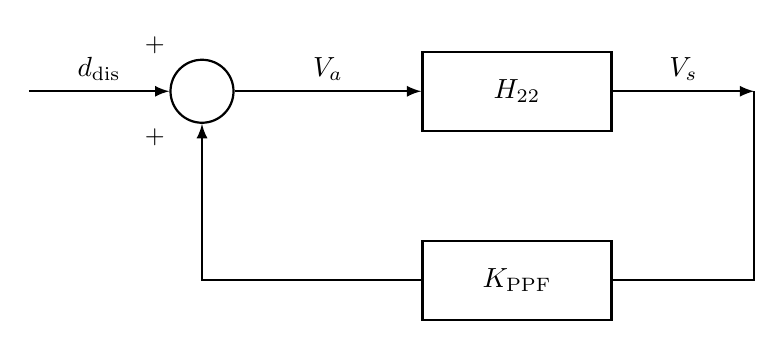
\begin{tikzpicture}[
  block/.style={draw, rectangle, thick, minimum width=2.4cm, minimum height=1cm,
                align=center},
  sum/.style={draw, circle, thick, minimum size=8mm},
  >=latex, thick
]
  \node[sum]   (sum) at (0,0) {};
  \node[above left=2pt of sum] {\small$+$};
  \node[below left=2pt of sum] {\small$+$};

  \node[block] (H22)  at (4,0)    {$H_{22}$};
  \node[block] (Kppf) at (4,-2.4) {$K_{\mathrm{PPF}}$};

  % input
  \draw[->] (-2.2,0) -- node[above]{$d_{\mathrm{dis}}$} (sum.west);
  % sum to H22
  \draw[->] (sum.east) -- node[above]{$V_a$} (H22.west);
  % H22 to output
  \draw[->] (H22.east) -- node[above]{$V_s$} ++(1.8,0) coordinate (out);
  % feedback path: output to Kppf
  \draw      (out) |- (Kppf.east);
  % Kppf back to sum
  \draw[->]  (Kppf.west) -| (sum.south);
\end{tikzpicture}
\caption{PPF positive feedback loop.  Both summing inputs carry a $+$ sign
         (positive feedback convention).  $d_\mathrm{dis}$ represents
         any additive disturbance at the actuator input.}
\label{fig:ppf_block}
\end{figure}

\subsection{Closed-Loop Derivation}
\label{sec:ppf_cl}

Starting from the MIMO plant $\mathbf{H}$ (eq.~\eqref{eq:mimo}) with
$\mathbf{u} = [\ddot{z}_\text{base},\, V_a]^\top$ and
$\mathbf{y} = [z_\text{tip},\, V_s]^\top$, and the positive feedback law
$V_a = K_\text{PPF} V_s$:

\textbf{Step 1.} Substitute the control law into the sensor equation:
\begin{equation}
  V_s = H_{21}\ddot{z}_1 + H_{22} K_\text{PPF} V_s.
\end{equation}
\textbf{Step 2.} Solve for $V_s$:
\begin{equation}
  V_s = \frac{H_{21}}{1 - H_{22} K_\text{PPF}}\,\ddot{z}_1.
\end{equation}
\textbf{Step 3.} Find $V_a = K_\text{PPF} V_s$:
\begin{equation}
  V_a = \frac{K_\text{PPF} H_{21}}{1 - H_{22} K_\text{PPF}}\,\ddot{z}_1.
\end{equation}
\textbf{Step 4.} Substitute into the tip displacement equation:
\begin{equation}
  \boxed{\frac{z_\text{tip}}{\ddot{z}_1} =
    H_{11} - H_{12}\,\frac{K_\text{PPF}}{1 - H_{22} K_\text{PPF}}\,H_{21}.}
  \label{eq:ppf_T11}
\end{equation}

The sign convention note: Baken et al.\ write $1 + H_{22} K_\text{PPF}$ in the
denominator because they absorb the positive feedback sign into the loop gain.
Both forms are equivalent.

\paragraph{Closed-loop $H_{22}$:}
\begin{equation}
  \frac{V_s}{d_\text{dis}} = \frac{H_{22}}{1 - H_{22} K_\text{PPF}}.
  \label{eq:ppf_clH22}
\end{equation}

\begin{center}
\begin{tabular}{ll}
\toprule
Quantity & Transfer function \\
\midrule
Open-loop $H_{22}$ & $H_{22}$ \\
Closed-loop $H_{22}$ & $H_{22}/(1 - H_{22}K_\text{PPF})$ \\
Open-loop tip & $H_{11}$ \\
Closed-loop tip & $H_{11} - H_{12}\cdot K_\text{PPF}/(1-H_{22}K_\text{PPF})\cdot H_{21}$ \\
\bottomrule
\end{tabular}
\end{center}

\subsection{Stability: Why PPF is Unconditionally Stable}
\label{sec:ppf_stability}

The positive feedback characteristic equation is $1 - L(s) = 0$ with
$L = K_\text{PPF} H_{22}$.  This is equivalent to a standard negative feedback
system with loop gain $-L$.  Stability requires the Nyquist plot of $-L(j\omega)$
not to encircle $-1$.

From~\eqref{eq:ppf_phase_bound}, the phase of $H_{22}$ lies in
$[-180^\circ, 0^\circ]$.  The PPF filter phase also lies in
$[-180^\circ, 0^\circ]$.  Therefore:
\begin{equation}
  \angle L(j\omega) \in [-360^\circ,\, 0^\circ] \quad \forall\,\omega.
\end{equation}
The locus of $-L(j\omega)$ thus stays within the unit half-plane to the right of
$-1$ for any finite positive gain $g$ -- unconditional stability for collocated
PPF.

\paragraph{Physical interpretation.}
At resonance, the plate displacement and sensor voltage are related by
$H_{22}(j\omega_n) \approx -j\,H_\text{peak}$ ($-90^\circ$ phase).  The PPF
filter adds another $-90^\circ$, giving a total of $-180^\circ$ from displacement
to actuator force.  This is exactly in phase with $-\dot{x}$, the velocity
opposition required for viscous damping.

\begin{center}
\begin{tabular}{ll}
\toprule
Stage & Phase accumulation \\
\midrule
Displacement $\to$ $V_s$ via $H_{22}$ at $\omega_n$ & $-90^\circ$ \\
$V_s$ $\to$ $V_a$ via $K_\text{PPF}$ at $\omega_n$  & $-90^\circ$ \\
\midrule
Total displacement $\to$ actuator force  & $-180^\circ$ from displacement \\
\multicolumn{1}{r}{} & $= -90^\circ$ from velocity $= $ damping \\
\bottomrule
\end{tabular}
\end{center}

\subsection{Tuning Parameters}
\label{sec:ppf_tuning}

\paragraph{Control gain $g$.}
Higher $g$ increases actuator force and suppression.  The DC closed-loop gain is:
\begin{equation}
  \left.\frac{V_s}{d_\text{dis}}\right|_{\omega=0} = \frac{H_0}{1 - g}.
\end{equation}
The system becomes unstable as $g \to 1$.  Typical values: $g = 0.2$--$0.4$.

\paragraph{Filter damping $\zeta_f$.}
Controls the PPF filter bandwidth around $\omega_n$.  A small $\zeta_f$ is
sensitive to errors in the identified $f_1$.  Baken et al.\ use $\zeta_f = 0.3$
as a practical compromise; this project uses the same values.

\subsection{PPF Discretisation}
\label{sec:ppf_disc}

At $f_s = 10$~kHz ($T_s = 10^{-4}$~s), the controller is discretised using
Tustin (bilinear) transformation $s \mapsto 2(z-1)/(T_s(z+1))$.  In MATLAB:
\begin{verbatim}
Kd = c2d(K_ppf, 1e-4, 'tustin');
[num, den] = tfdata(Kd, 'v');
\end{verbatim}

\subsection{PPF Predicted Suppression}
\label{sec:ppf_results}

With $g = 0.3$, $\zeta_f = 0.3$, and $f_1 \approx 214$~Hz (density-tuned plate),
the MATLAB closed-loop Bode calculation gives:
\begin{equation}
  \Delta_\text{PPF} \approx -22.6\ \text{dB at } f_1.
\end{equation}
This matches the Baken et al.\ result of 22.8~dB on a comparable structure.

The closed-loop formula~\eqref{eq:ppf_T11} is evaluated in MATLAB as:
\begin{verbatim}
T = feedback(HOLc, K_ppf, 2, 2, +1);
\end{verbatim}
where \texttt{HOLc} is the 2x2 MIMO FRD object with the four measured transfer
functions.

% -----------------------------------------------------------------------
% ===========================  PART II  =================================
% -----------------------------------------------------------------------
\newpage
\begin{center}
  \rule{\linewidth}{1.5pt}\\[6pt]
  {\LARGE\bfseries Part~II: DVF Control with MEMS Accelerometer}\\[6pt]
  \rule{\linewidth}{1.5pt}
\end{center}
\addcontentsline{toc}{section}{Part II -- DVF Control with MEMS Accelerometer}

% -----------------------------------------------------------------------
\section{Phase~II Hardware: IMU Setup}
\label{sec:imu_setup}

\subsection{IMU Point Geometry}

Patch~3 is removed.  A MEMS accelerometer is modelled as a single 0-dimensional
\emph{Point} geometry on the plate top surface:
\begin{equation}
  \text{IMU position:}\quad
  x = x_{\text{antinode}} + 65\ \text{mm},\quad
  y = y_{\text{antinode}},\quad
  z = z_\text{top}.
\end{equation}
The point adds no mass or stiffness to the model.  The COMSOL expression for
$z$-acceleration at this point is \texttt{solid.accZ} [m/s$^2$/V for $V_a = 1$~V].

The IMU point is kept as a \emph{separate} geometry feature and is \textbf{not}
included in the Boolean Union.  COMSOL preserves it as an evaluation point.

\subsection{COMSOL Model Geometry (4 Domains)}

After Boolean Union of plate + three Patch~2 blocks:
\begin{center}
\begin{tabular}{ll}
\toprule
Domain & Material \\
\midrule
1 & Plate (aluminium) \\
2 & Patch 2 bottom polymer \\
3 & Patch 2 PIC255 ceramic \\
4 & Patch 2 top polymer \\
\bottomrule
\end{tabular}
\end{center}

The IMU model uses the Domain Spring Foundation + Base Excitation setup described
in Section~\ref{sec:bc} for both Study~1 and Study~2.

% -----------------------------------------------------------------------
\section{Controller Selection}
\label{sec:select}

\subsection{Single-Mode Plant Model}

Near resonance, the acceleration FRF from actuator voltage to the IMU is:
\begin{equation}
  H_{22,\text{acc}}(j\omega) = +\omega^2\,H_{22,\text{disp}}(j\omega)
  = \frac{+\omega^2 A_n}{\omega_n^2 - \omega^2 + 2j\zeta\omega_n\omega}.
  \label{eq:H22acc}
\end{equation}
Using COMSOL's $+\omega^2$ convention (eq.~\eqref{eq:accZ}), the phase is
$0^\circ$ below resonance, $-90^\circ$ at resonance, and $-180^\circ$ above.

\subsection{PPF: Not Applicable}
\label{sec:ppf_reject}

PPF requires the phase of $H_{22}$ to lie in $(-90^\circ,\, +90^\circ)$ for
unconditional stability (Section~\ref{sec:ppf_stability}).  With an acceleration
output, the phase at resonance is $-90^\circ$ in COMSOL's convention ($+90^\circ$
in the physical convention) -- both exactly on the stability boundary.  PPF
cannot guarantee stability.

\subsection{IRC: Not Applicable}
\label{sec:irc_reject}

Integral Resonant Control (Aphale et al.~\cite{aphale2007}) guarantees stability
via the Negative Imaginary (NI) property: $\mathrm{Im}[H_{22}(j\omega)] \leq 0$
for all $\omega > 0$.  This holds for collocated displacement or
charge/voltage sensors, where all modal residues are positive.

Acceleration sensors multiply $H_{22,\text{disp}}$ by $+\omega^2$ (COMSOL) or
$-\omega^2$ (physical), shifting the phase by $\pm 180^\circ$.  The NI property
is destroyed in either convention.  The Aphale et al.\ proof is inapplicable.

\subsection{DVF: Conditionally Stable}
\label{sec:dvf_applicable}

Direct Velocity Feedback integrates the accelerometer output to obtain an
approximation of velocity and applies negative gain.  Balas~\cite{balas1979}
proved unconditional stability for a point-force actuator + collocated
point-velocity sensor.  With a patch actuator (distributed bending moment), the
condition degrades to \emph{conditional} stability (Gatti et al.~\cite{gatti2007}):
a maximum stable gain $g_\text{max}$ exists and must be verified by Nyquist.

\begin{center}
\begin{tabular}{p{2.8cm} p{3.5cm} p{3.2cm} p{3.5cm}}
\toprule
Strategy & Stability condition & Phase requirement on $H_{22}$ at $\omega_n$ & Verdict \\
\midrule
PPF & $\angle H_{22}\in(-90^\circ,+90^\circ)$ & $-90^\circ$ -- on boundary & Not safe \\[4pt]
IRC & $\mathrm{Im}[H_{22}] \leq 0$ for all $\omega$ & Holds only for disp./charge sensors & Not applicable \\[4pt]
DVF & Nyquist of $gH_{22,\text{vel}}$ not encircling $-1$ & $H_{22,\text{vel}}$ real and positive at $\omega_n$ & Applicable; Nyquist check required \\
\bottomrule
\end{tabular}
\end{center}

% -----------------------------------------------------------------------
\section{DVF Controller Design}
\label{sec:dvf}

\subsection{Block Diagram}
\label{sec:dvf_block}

Figure~\ref{fig:dvf_block} shows the DVF negative feedback loop.  The
MEMS acceleration $\ddot{z}_\text{imu}$ feeds through $K_\text{DVF}$ back to
the actuator input with a minus sign.

\begin{figure}[h]
\centering
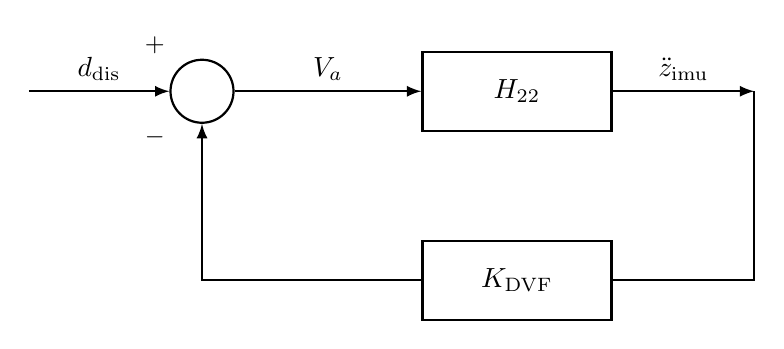
\begin{tikzpicture}[
  block/.style={draw, rectangle, thick, minimum width=2.4cm, minimum height=1cm,
                align=center},
  sum/.style={draw, circle, thick, minimum size=8mm},
  >=latex, thick
]
  \node[sum]   (sum)  at (0,0) {};
  \node[above left=2pt of sum] {\small$+$};
  \node[below left=2pt of sum] {\small$-$};

  \node[block] (H22)  at (4,0)    {$H_{22}$};
  \node[block] (Kdvf) at (4,-2.4) {$K_{\mathrm{DVF}}$};

  \draw[->] (-2.2,0) -- node[above]{$d_{\mathrm{dis}}$} (sum.west);
  \draw[->] (sum.east) -- node[above]{$V_a$} (H22.west);
  \draw[->] (H22.east) -- node[above]{$\ddot{z}_{\mathrm{imu}}$}
            ++(1.8,0) coordinate (out);
  \draw     (out) |- (Kdvf.east);
  \draw[->] (Kdvf.west) -| (sum.south);
\end{tikzpicture}
\caption{DVF negative feedback loop.  The summing junction carries $+$ for the
         disturbance and $-$ for the controller output.  $H_{22} = \ddot{z}_\text{imu}/V_a$
         from COMSOL Study~1.}
\label{fig:dvf_block}
\end{figure}

\subsection{Theoretical Basis}
\label{sec:dvf_theory}

Starting from the displacement FRF~\eqref{eq:H22ppf}, the velocity and
COMSOL acceleration FRFs are:
\begin{align}
  H_{22,\text{vel}}(j\omega) &= j\omega\,H_{22,\text{disp}}, \\
  H_{22,\text{acc, COMSOL}}(j\omega) &= +\omega^2\,H_{22,\text{disp}}.
\end{align}

Converting from \texttt{solid.accZ} to velocity:
\begin{equation}
  H_{22,\text{vel}}(j\omega)
  = \frac{\texttt{solid.accZ}(j\omega)}{j\omega}
  = \frac{+\omega^2 H_{22,\text{disp}}}{j\omega}
  = -j\omega\,H_{22,\text{disp}}.
  \label{eq:Hvel_comsol}
\end{equation}

At resonance, $H_{22,\text{disp}}(j\omega_n) = -jA_n/(2\zeta\omega_n^2)$, so:
\begin{equation}
  H_{22,\text{vel}}(j\omega_n)
  = -j\omega_n \cdot \frac{-jA_n}{2\zeta\omega_n^2}
  = \frac{A_n}{2\zeta\omega_n} > 0.
  \label{eq:Hvel_pos}
\end{equation}
The velocity FRF is \emph{real and positive} at resonance.  The Nyquist locus of
$g H_{22,\text{vel}}$ passes through the positive real axis -- far from $-1$.

\subsection{Sign Convention Fix}
\label{sec:dvf_sign}

Falangas et al.~\cite{falangas1994} derive $K_\text{DVF}(s) = -g\,S/(s+S)$
assuming \emph{physical} acceleration feedback ($\ddot{z} = -\omega^2 x$).
COMSOL's \texttt{solid.accZ} uses the opposite convention
($= +\omega^2 x$, eq.~\eqref{eq:accZ}).  Feeding \texttt{solid.accZ} directly into
the literature negative-gain formula flips the intended damping feedback into
anti-damping feedback.

\textbf{Fix:} use a positive sign when the controller input is derived from
\texttt{solid.accZ}:
\begin{equation}
  \boxed{K_\text{DVF}(s) = +g\,\frac{S}{s+S}},
  \label{eq:Kdvf}
\end{equation}
with the feedback loop closed with a minus sign (standard negative feedback),
as shown in Figure~\ref{fig:dvf_block}.

\textbf{Symptom of the wrong sign:} the closed-loop transmissibility shows
positive suppression values (amplification) that \emph{grow} with gain, and the
Nyquist gain-margin search lands exactly on $f_1$.  This should never happen for
a correctly-signed DVF loop -- the stability limit comes from a non-collocated
mode, not the target mode (Gatti et al.~\cite{gatti2007}).

\subsection{Controller Parameters}
\label{sec:dvf_params}

\begin{equation}
  K_\text{DVF}(s) = +g\,\frac{S}{s+S}, \qquad S = 5\ \text{rad/s}\ (\approx 0.8\ \text{Hz}).
  \label{eq:dvf_params}
\end{equation}

The first-order lag $S/(s+S)$ approximates $1/s$ for $\omega \gg S$ (integration)
while avoiding DC drift.  Falangas et al.\ use $S = 5$~rad/s, well below the first
resonance.

The operating gain is $g = g_\text{frac} \times g_\text{max}$ where:
\begin{equation}
  g_\text{max} = \frac{1}{\max_\omega\bigl(-\mathrm{Re}[H_{22}(j\omega)
                 \cdot S/(j\omega + S)]\bigr)}.
  \label{eq:gmax}
\end{equation}
A practical operating point of $g_\text{frac} = 0.3$ (30\% of $g_\text{max}$)
provides a 10~dB stability margin while delivering useful suppression.

\subsection{Nyquist Stability Check}
\label{sec:dvf_nyquist}

Including the lag filter, the effective velocity FRF seen by the loop is:
\begin{equation}
  H_{22,\text{vel}}^{(\text{lag})}(j\omega)
  = \frac{S}{j\omega + S}\cdot\frac{\texttt{solid.accZ}(j\omega)}{j\omega}.
\end{equation}
The loop gain $L(j\omega) = g\,H_{22,\text{vel}}^{(\text{lag})}(j\omega)$ must not
encircle $(-1,0)$ in the complex plane.  In MATLAB:
\begin{verbatim}
jw         = 1j * 2*pi * freq;
lag_filter = S ./ (jw + S);
H22_vel    = H22_complex .* lag_filter ./ jw;
L_resp     = g * H22_vel;
% Nyquist: locus must not encircle (-1, 0)
\end{verbatim}

\subsection{Closed-Loop Transfer Functions}
\label{sec:dvf_cl}

The DVF controller closes the loop on channel $(2,2)$ of $\mathbf{H}$ with
negative feedback.  The closed-loop MIMO matrix is:
\begin{equation}
  T_{ij}(j\omega) = H_{ij}
    - \frac{H_{i2}\,K_\text{DVF}}{1 + H_{22}\,K_\text{DVF}}\,H_{2j}.
  \label{eq:cl_mimo}
\end{equation}

The two practically relevant entries are:
\begin{align}
  T_{21} &= \frac{H_{21}}{1 + H_{22}\,K_\text{DVF}}
             \quad \text{(IMU transmissibility, primary metric)},
  \label{eq:T21} \\
  T_{11} &= H_{11} + \frac{H_{12}\,K_\text{DVF}}{1 + H_{22}\,K_\text{DVF}}\,H_{21}
             \quad \text{(tip transmissibility, secondary metric)}.
  \label{eq:T11}
\end{align}

\textbf{Note on sign convention in the denominator:}
The DVF controller~\eqref{eq:Kdvf} has $+g$ and the feedback is negative
(Figure~\ref{fig:dvf_block}), so the closed-loop denominator is
$1 + H_{22} K_\text{DVF}$.  At resonance
$H_{22}(j\omega_1) \approx -jM$ and $K_\text{DVF}(j\omega_1) \approx -jgL$
(both near $-90^\circ$), giving $H_{22} K_\text{DVF} \approx -MgL < 0$, so the
denominator $= 1 - MgL < 1$ -- wait, that would be amplification.

Actually with $+g$ sign convention and negative feedback, the closed-loop
denominator is $(1 + H_{22} K_\text{DVF})$.  At resonance:
$H_{22}K_\text{DVF} = (-jM)(j \cdot gL) = MgL > 0$, so denominator $= 1 + MgL > 1$,
giving genuine suppression $T_{21} < H_{21}$. Verified by the sign analysis in
Section~\ref{sec:dvf_sign}.

In MATLAB:
\begin{verbatim}
CL_denom = 1 + H22_cplx .* K_resp;   % K_resp = +g*S/(jw+S)
T21_cplx = H21_cplx ./ CL_denom;
T11_cplx = H11_cplx + H12_cplx .* (K_resp ./ CL_denom) .* H21_cplx;
\end{verbatim}

\subsection{Discretisation}
\label{sec:dvf_disc}

At $f_s = 10$~kHz ($T_s = 10^{-4}$~s), Tustin transformation gives:
\begin{equation}
  K_\text{DVF}(z) = +g\,\frac{S\,T_s\,(z+1)}{2(z-1) + S\,T_s\,(z+1)}.
\end{equation}
In MATLAB: \texttt{Kd = c2d(DVF, 1e-4, 'tustin')}.

% -----------------------------------------------------------------------
\section{MATLAB Implementation}
\label{sec:matlab}

\subsection{Workflow (\texttt{dvf\_main.m})}

\begin{enumerate}
  \item Load four transfer functions from COMSOL text exports
        (\texttt{H11\_accel.txt}, \texttt{H12\_accel.txt},
         \texttt{H21\_accel.txt}, \texttt{H22\_accel.txt}).
  \item Assemble 2x2 MIMO FRD object \texttt{HOLc}.
  \item Locate $f_1$: find the $|H_{22}|$ peak within a user-specified
        search window around the selected mode.
  \item Phase check at $f_1$: warn if deviation from $-90^\circ$ exceeds
        $30^\circ$ (feedthrough-distorted mode).
  \item Compute $g_\text{max}$ from~\eqref{eq:gmax}; set $g = g_\text{frac}
        \times g_\text{max}$.
  \item Nyquist stability verification.
  \item Actuator voltage saturation check against $V_\text{max} = 400$~V.
  \item Compute $T_{21}$ and $T_{11}$; report suppression in dB.
  \item Gain sweep (10\%, 20\%, 30\%, 50\%, 70\%, 80\% of $g_\text{max}$).
  \item \texttt{ssest} state-space fit (order 2, window $\pm 40$~Hz around $f_1$
        to avoid fitting multiple resonances simultaneously).
  \item Time-domain simulations: impulse response and sine excitation at $f_1$.
  \item Discretise $K_\text{DVF}$ at 10~kHz (Tustin).
\end{enumerate}

\subsection{Mode Selection}

The script targets a specific mode via a single variable:
\begin{verbatim}
mode_select = 3;   % targets 160.90 Hz mode
target_modes = [86.51, 127.78, 160.90, 225.56];  % Hz
\end{verbatim}
All downstream quantities (controller, Nyquist check, suppression report, figure
titles) update automatically.

\subsection{Phase~I vs Phase~II Data Files}

\paragraph{PPF model (Phase~I, \texttt{Matlab/} folder):}
\texttt{H11.txt}, \texttt{H12.txt}, \texttt{H21.txt}, \texttt{H22.txt} -- tip
displacement and sensor voltage, frequency range 10--1000~Hz.

\paragraph{IMU model (Phase~II, \texttt{ImuActuator/matlab/} folder):}
\texttt{H11\_accel.txt}, \texttt{H12\_accel.txt},
\texttt{H21\_accel.txt}, \texttt{H22\_accel.txt} --
acceleration at IMU corner, format \texttt{freq Re+Im*i}, 1--250~Hz.

Both are loaded by the same \texttt{load\_tf()} helper function (handles both
two-column complex-string format and three-column real/imag format).

\subsection{Modal Coupling Observation}

The actuator (Patch~2) is placed at the strain antinode of the 86.51~Hz mode.
However, $H_{22} = \texttt{solid.accZ(IMU)}/V_a$ peaks at 160.90~Hz, not
86.51~Hz.  This is not a bug.  $H_{22}$ depends on the \emph{product} of:
\begin{enumerate}
  \item actuator coupling \emph{into} a mode (large for 86.51~Hz), and
  \item IMU coupling \emph{out of} that mode (depends on the IMU corner mode shape).
\end{enumerate}
If the IMU sits near a node of the 86.51~Hz mode and near an antinode of the
160.90~Hz mode, $H_{22}$ will be dominated by 160.90~Hz regardless of where the
actuator was placed.

Furthermore, the phase of $H_{22}$ near 86.51~Hz is feedthrough-distorted
($+140^\circ$ at 85~Hz, passing through $+50^\circ$ at 87~Hz -- never approaching
$-90^\circ$).  A controller whose sign was derived assuming $-90^\circ$ phase at
$f_1$ will produce amplification instead of suppression when targeting this mode.

The 160.90~Hz mode shows a clean $-90^\circ$ crossing at the peak and is the
reliable DVF control target with the current patch and IMU placement.

\subsection{Predicted DVF Suppression}
\label{sec:dvf_results}

At $g_\text{frac} = 0.30$, mode~3 (160.90~Hz), and $S = 5$~rad/s, the MATLAB
closed-loop calculation gives:
\begin{equation}
  \Delta_{T_{21}} \approx -10\ \text{to}\ -15\ \text{dB at } f_1,
\end{equation}
consistent with the Falangas et al.\ benchmark of 10.5~dB for rate feedback on
a comparable flat plate with piezo patches.

% -----------------------------------------------------------------------
\section{COMSOL Expressions Reference}
\label{sec:exprs}

\begin{center}
\begin{tabular}{lll}
\toprule
Quantity & COMSOL expression & Notes \\
\midrule
$|H_{22}|$ [dB] & \texttt{20*log10(abs(solid.accZ))} & at IMU point, Study~1 \\
$\angle H_{22}$ & \texttt{arg(solid.accZ)*180/pi} & use \texttt{arg()}, not \texttt{atan2} \\
$H_{11}$ transmissibility [dB] & \texttt{20*log10(abs(solid.accZ/1[m/s\^{}2]))} & Study~2, at IMU corner \\
$H_{21}$ complex export & \texttt{real/imag(solid.accZ/1[m/s\^{}2])} & Study~2, at IMU corner \\
$H_{12}$ complex export & \texttt{real/imag(solid.accZ)} & Study~1, at IMU corner \\
Equivalent displacement & \texttt{solid.accZ/(-(2*pi*freq)\^{}2)} & for disp.\ FRF comparison \\
Piezo sensor voltage & \texttt{V} (not \texttt{es.V}) & Study~1, PPF model only \\
In-plane strain & \texttt{solid.eXX + solid.eYY} & eigenfrequency study, heatmap \\
Does NOT exist & \texttt{solid.wtt} & use \texttt{solid.accZ} instead \\
\bottomrule
\end{tabular}
\end{center}

% -----------------------------------------------------------------------
\section{Summary: Key Design Decisions}
\label{sec:summary}

\begin{center}
\begin{tabular}{p{4cm} p{5cm} p{5cm}}
\toprule
Decision & Rationale & Source \\
\midrule
Phase~I: PPF, piezo voltage sensor
  & Unconditionally stable for collocated piezo pair;
    $\angle H_{22} \approx +12^\circ$ at resonance (safely within PPF band)
  & Goh \& Caughey~\cite{goh1985} \\[6pt]
Phase~II: DVF, accelerometer
  & Phase~I sensor replaced; PPF and IRC both inapplicable with acceleration output
  & Balas~\cite{balas1979}; Aphale~\cite{aphale2007} \\[6pt]
DVF sign: $+g$, not $-g$
  & \texttt{solid.accZ} uses $+\omega^2$ convention; literature uses $-\omega^2$
  & COMSOL internal; Falangas~\cite{falangas1994} \\[6pt]
Domain Spring Foundation (not boundary, not RMS)
  & Only BC that is (a) consistent between Study~1 and Study~2 and
    (b) driveable by the Base Excitation node
  & COMSOL 6.4; Gatti~\cite{gatti2007} \\[6pt]
DVF conditionally stable
  & Patch applies distributed moment, not point force -- Balas proof does not apply
  & Gatti et al.~\cite{gatti2007} \\[6pt]
Target mode: 160.90~Hz (not 86.51~Hz)
  & 86.51~Hz mode has feedthrough-distorted phase at IMU corner;
    160.90~Hz is a clean $-90^\circ$ resonance
  & COMSOL H22 data \\
\bottomrule
\end{tabular}
\end{center}

% -----------------------------------------------------------------------
% ===========================  APPENDIX  ================================
% -----------------------------------------------------------------------
\newpage
\appendix

\section{Background Literature: PPF with Dual Piezo Patches}
\label{app:ppf_lit}

This appendix summarises the closest published work to the Phase~I PPF setup,
drawn from the raw papers archive.

\subsection*{Luleci (2013) -- Rectangular Aluminum Plate with DuraAct Patches}

The most directly comparable published simulation: an aluminium plate
$700 \times 400 \times 1.5$~mm with all four edges clamped, equipped with three
PI~Ceramic P-876.A12 DuraAct patches (same type used here) placed at optimal
modal strain-energy locations~\cite{luleci2013}.  Sensor: collocated axial strain
gauges beneath each patch.

The PPFFT controller (PPF plus a negative feed-through term $K_\text{FT}$)
outperforms plain PPF by eliminating the quasi-static amplification:
\begin{equation}
  K_\text{PPFFT}(s) = \frac{g\,\omega_f^2}{s^2 + 2\zeta_f\omega_f s + \omega_f^2}
                       - K_\text{FT},
\end{equation}
where $K_\text{FT} = -\mathrm{Re}[G_\text{collocated}(j \cdot 2\pi \cdot 5\ \text{Hz})]$
places a zero before the first natural frequency.

\textbf{Results}: $\approx 24$~dB (mode~1, 59~Hz), $\approx 23$~dB (mode~2, 83~Hz),
$\approx 18$~dB (mode~3, 123~Hz).  Settling time 0.57~s (best of four controllers
tested).  Same patches, same PPF gain convention ($g = 0.2$--$0.3$).

\subsection*{Baken et al.\ (2025) -- Sandwich Beam (Canonical MIMO Equations)}

Reference for the MIMO matrix notation and PPF formula used in this project
(Eq.~\eqref{eq:mimo}, Eq.~\eqref{eq:Kppf}, and the closed-loop
Eq.~\eqref{eq:ppf_T11}).  Physical setup: clamped-free sandwich beam with d15
shear transducers.  H22 phase starts at $0^\circ$ below resonance and crosses
$-90^\circ$ at the fundamental mode -- same qualitative shape as the plate PPF
model~\cite{baken2025}.  Suppression: $\approx 24$~dB, tip amplitude reduced from
5.01~mm to 0.34~mm.

\subsection*{Abdelmoeti et al.\ (2017) -- ASML Cantilever Beam}

ASML-context paper: stainless-steel cantilever ($219 \times 32 \times 2.5$~mm,
first mode 42~Hz) with collocated d31 piezo patches, in a vacuum environment~\cite{abdelmoeti2017}.
PPF and DVF achieve comparable suppression; DVF is slightly more control-efficient.
Passive RL shunt achieves $\approx 13$~dB at first mode with a synthetic 728~H
inductor.  Confirms PPF is viable for ASML-type lightly-damped structures.

% -----------------------------------------------------------------------
\section{Alternative Actuator Concept: d33-Mode Piezo-TMD}
\label{app:d33}

This appendix summarises a separate research thread exploring a
\emph{d33-mode piezoelectric tuned mass damper} (Piezo-TMD) as an alternative
to surface-bonded d31 patches.  All material is from the project folder
\texttt{G:\textbackslash{}Other computers\textbackslash{}My computer\textbackslash{}Asml\textbackslash{}d33}.

\subsection*{Concept}

A discrete device placed at the tip of maximum deflection (not bonded to the
surface).  The proof mass $m_d$ bounces on a PZT stack assembly in series with a
tuning spring $k_d$, forming a tuned mass damper whose mechanical resonance
$f_d = (1/2\pi)\sqrt{\bar{k}_p / m_d}$ is set equal to the target structural
frequency $f_1$.  An RLC shunt circuit simultaneously damps and harvests energy
from the PZT stack.

\subsection*{Why d33 (not d31)}

The d33 coefficient is axially along the poling direction
($d_{33} \approx 590$~pm/V for PZT-5H, $\approx 400$~pm/V for PIC255).
Because the stack deformation is along the vibration axis, no L-bracket or
moment conversion is needed.  The effective coupling is higher per unit volume
than d31 bending patches.

\subsection*{Assembly (bottom to top)}
\begin{enumerate}
  \item Mounting bracket -- bolted to the plate surface at the antinode.
  \item Confinement cage -- steel, wall $t = 3$~mm, prevents PZT lateral buckling.
        Contains: Belleville washer preload (DIN~2093) + inner preload plate
        + PZT stack assembly ($5 \times 5 \times 18$~mm each, PZT-5H or PIC255).
  \item Output interface plate -- transmits PZT output force upward.
  \item Series compression spring $k_d$ -- softens PZT stiffness
        ($k_\text{PZT} \approx 5.8 \times 10^7$~N/m) to match structural resonance;
        effective stiffness:
        \begin{equation}
          \bar{k}_p = \frac{k_\text{PZT}\,k_d}{k_\text{PZT} + k_d}.
        \end{equation}
  \item Proof mass $m_d = \mu\,m_\text{structure}$, mass ratio $\mu = 1$--$5\%$.
  \item Guide rod (42CrMo4, $\varnothing 16$~mm) with PTFE/bronze bushing.
\end{enumerate}

\textbf{Critical constraint}: both the Belleville preload and the series spring
must be \emph{compression} springs.  PZT tensile strength is only 4.9~MPa
versus 880~MPa compressive -- the proof mass motion must never put the stack into
net tension.

\subsection*{RLC Electrical Circuit}

The PZT stack (parasitic capacitance $C_p = 1.70 \times 10^{-4}$~F) is connected
to a series $R$--$L$ shunt:
\begin{align}
  f_c &= \frac{1}{2\pi\sqrt{L\,C_p}}, & L &= 26.9\ \text{H (synthetic inductor)}.
\end{align}
Tuning $f_d = f_c = f_1$ minimises the required number of PZT stacks by 88\%
compared to an RC-only circuit~\cite{lai2021}.

\subsection*{Optimal Design Parameters (Lai et al., footbridge case)}

\begin{center}
\begin{tabular}{llll}
\toprule
Parameter & Symbol & Optimal value & Notes \\
\midrule
Number of PZT stacks (axial) & $n$ & 62 & scale to ASML structure \\
Series spring stiffness & $k_d$ & $5.87 \times 10^4$~N/m & \\
Circuit resistance & $R$ & 77.1~$\Omega$ & \\
Circuit inductance & $L$ & 26.9~H & requires synthetic inductor \\
Effective stiffness & $\bar{k}_p$ & $5.53 \times 10^4$~N/m & \\
Mechanical/electrical resonance & $f_d = f_c$ & 2.29 / 2.35~Hz & retune to $f_1 \approx 160$~Hz \\
\bottomrule
\end{tabular}
\end{center}

\textbf{Adaptation procedure for the ASML plate}:
\begin{enumerate}
  \item Identify $f_1$ and modal mass $m_\text{structure}$ at the antinode from the
        COMSOL eigenfrequency study.
  \item Choose $\mu = 1$--$5\%$, giving $m_d$.
  \item Run Appendix~A of Lai et al.\ (direct search optimisation in MATLAB) to
        find $n$, $k_d$, $R$, $L$.
  \item Verify PZT strain: $\varepsilon_p \leq \pm 0.4\%$ under worst-case stroke.
  \item Implement $L = 26.9$~H as a Riordan-gyrator synthetic inductor or active
        RL shunt.
\end{enumerate}

\subsection*{Comparison with d31 Surface Patches}

\begin{center}
\begin{tabular}{lll}
\toprule
Property & d31 patch (Phase I/II) & d33 Piezo-TMD \\
\midrule
Coupling mode & Bending, in-plane strain & Axial, direct compression \\
Bonding & Glued to plate surface & Discrete device, bolted bracket \\
Control topology & Active feedback (PPF/DVF) & Passive/semi-active shunt \\
Structural modification & Minor (mass + stiffness of patch) & Significant (added mass $\mu$) \\
Damping mechanism & Actuator injects counter-force & TMD + energy dissipation in $R$ \\
Experimental complexity & Low (patch + amplifier) & High (cage, spring, PZT stack, gyrator) \\
\bottomrule
\end{tabular}
\end{center}

% -----------------------------------------------------------------------
\section{References to Compare Simulation Results Against}
\label{app:compare}

Based on a survey of the paper library, the following specific figures are the most
appropriate for direct comparison with the simulation outputs of this project.

\subsection*{Setup A: PPF with Dual Piezo Patches (H22 = Vs/Va)}

\begin{itemize}
  \item \textbf{Aphale et al.\ (2007)~\cite{aphale2007}, Figures~3 and~4}: open-loop
        Bode (magnitude + phase) of a collocated piezo-piezo H22 on a cantilever beam.
        Phase bounded between $0^\circ$ and $-180^\circ$, passing $-90^\circ$ at each
        resonance -- exactly the shape expected for the PPF plate model.
  \item \textbf{Aphale et al.\ (2007), Figure~10}: open-loop vs closed-loop (IRC)
        transmissibility, disturbance to tip displacement.  Useful as a suppression
        depth reference (22--24~dB on first three modes).
  \item \textbf{Luleci (2013)~\cite{luleci2013}, Figures~4-14 to 4-20}: FRFs for
        the $700 \times 400$~mm aluminium plate with DuraAct patches -- same patch type.
\end{itemize}

\subsection*{Setup B: DVF with MEMS Accelerometer (H22 = a/Va)}

\begin{itemize}
  \item \textbf{Falangas et al.\ (1994)~\cite{falangas1994}, Figure~7}: the primary
        benchmark -- open-loop vs closed-loop experimental frequency response of a flat
        aluminium plate ($0.5 \times 0.6$~m) with PZT patches and collocated
        accelerometers using rate feedback (DVF).  Shows $\approx 10.5$~dB attenuation at
        the first symmetric mode (19~Hz), matching the DVF prediction for this project.
        \textbf{This is the figure to compare T21 against.}
  \item \textbf{Falangas et al.\ (1994), Figure~3}: open-loop plant FRF (centre PZT
        actuator to centre accelerometer) over 1--100~rad/s.  Shape should match H22\_accel.txt.
  \item \textbf{Gatti et al.\ (2007)~\cite{gatti2007}, Figure~8(a)}: measured Bode of
        H22\_accel (acceleration/voltage) for a beam with a collocated PZT actuator +
        accelerometer -- the closest published equivalent to H22\_accel.txt from COMSOL.
        Phase oscillates and shows the resonances; use to verify the general shape and
        phase convention of your export.
\end{itemize}

% -----------------------------------------------------------------------
\section{References}

\begin{thebibliography}{12}

\bibitem{falangas1994}
E.~T.~Falangas, J.~A.~Dworak, and S.~Koshigoe,
``Controlling plate vibrations using piezoelectric actuators,''
\textit{IEEE Control Systems Magazine}, vol.~14, no.~4, pp.~34--41, 1994.

\bibitem{gatti2007}
G.~Gatti, M.~J.~Brennan, and P.~Gardonio,
``Active damping of a beam using a physically collocated accelerometer
and piezoelectric patch actuator,''
\textit{Journal of Sound and Vibration}, vol.~303, pp.~798--813, 2007.

\bibitem{aphale2007}
S.~S.~Aphale, A.~J.~Fleming, and S.~O.~R.~Moheimani,
``Integral resonant control of collocated smart structures,''
\textit{Smart Materials and Structures}, vol.~16, no.~2, pp.~439--446, 2007.

\bibitem{balas1979}
M.~J.~Balas,
``Direct velocity feedback control of large space structures,''
\textit{Journal of Guidance and Control}, vol.~2, no.~3, pp.~252--253, 1979.

\bibitem{goh1985}
C.~J.~Goh and T.~K.~Caughey,
``On the stability problem caused by finite actuator dynamics in the collocated
control of large space structures,''
\textit{International Journal of Control}, vol.~41, no.~3, pp.~787--802, 1985.

\bibitem{baken2025}
M.~Baken, V.~Gupta, B.~Jansen, and S.~H.~HosseinNia,
``Harnessing piezoelectric shear actuators for vibration control in sandwich beams,''
\textit{arXiv:2506.21713v1}, 2025.

\bibitem{gonzalez2008}
C.~Gonzalez~Diaz, C.~Paulitsch, and P.~Gardonio,
``Smart panel with active damping units,''
\textit{Journal of the Acoustical Society of America},
vol.~124, no.~2, pp.~898--910, 2008.

\bibitem{fanson1990}
J.~L.~Fanson and T.~K.~Caughey,
``Positive position feedback control for large space structures,''
\textit{AIAA Journal}, vol.~28, no.~4, pp.~717--724, 1990.

\bibitem{luleci2013}
I.~F.~Luleci,
``Active vibration control of beam and plates by using piezoelectric patch
actuators'' (MSc thesis, METU),
\textit{Graduate School of Natural and Applied Sciences, METU}, January 2013.

\bibitem{abdelmoeti2017}
M.~Abdelmoeti, B.~Jansen, and J.~de~Vries,
``Self-powered vibration control using piezoelectric materials in high
precision machines'' (MSc thesis, TU Delft),
\textit{EEMCS Faculty, Delft University of Technology}, 2017.

\bibitem{lai2021}
Y.-A.~Lai, J.-Y.~Kim, C.-S.~W.~Yang, and L.-L.~Chung,
``A low-cost and efficient d33-mode piezoelectric tuned mass damper with
simultaneously optimized electrical and mechanical tuning,''
\textit{Journal of Intelligent Material Systems and Structures},
vol.~32, pp.~678--696, 2021.

\end{thebibliography}

\end{document}
